\documentclass{beamer}

%\beamertemplatesolidbackgroundcolor{black!5}
%\beamertemplatetransparentcovered

\usepackage[english,german]{babel}

\usepackage{amsmath}
\usepackage{amssymb}

\usepackage{graphicx}

\graphicspath{ {./rsc/} }

\setbeamertemplate{frametitle}[default][center]

\title{Parallelisierung in Computer Vision}
\subtitle{Grundlagen mit Implementierungsbeispielen}

\author[Braun]{Christian Braun}

\begin{document}

\begin{frame}
  \titlepage
\end{frame}

\begin{frame}<1>
  \frametitle{Motivation}
  \framesubtitle{ein kurzer Überblick}
  
  \begin{itemize}
    \item Erste Sichtung von parallelisierbarer Lösungen
    \item Merkmale um die Parallelisierbarkeit einzuschätzen
    \item Mögliche Implementierungsbeispiele
    \item Probleme aus der Praxis
  \end{itemize}
  
\end{frame}

\begin{frame}<2>
  \frametitle{Konventationen bezüglich Computer Vision}
  \framesubtitle{Um eine gemeinsame Grundlage zu schaffen}
  \begin{itemize}
    \item Abbildungsfunktionen können ein n-Tupel auf ein m-Tupel abbilden, mit n,m $\in \mathbb{N}$
    \item Ein Tupel besteht aus einer Matrix(c,r) von Pixeln, für die n = c*r gilt mit c,r $\in \mathbb{N} \&$ c,r $\geq$ 1
    \item Ein Pixel ist ein 3-wertiges Skalar welches die Farben in Reihenfolge Blau, Grün und Rot darstellt (BGR Farbraum)
    \item Ein (Kamera-)Bild ist eine Matrix(c,r) 
  \end{itemize}
\end{frame}

\begin{frame}<3>
  \frametitle{Korrektur von Abbildungsfehlern}
  \framesubtitle{}
  
  \begin{center}
    \begin{table}[]
      \begin{tabular}{cc}
        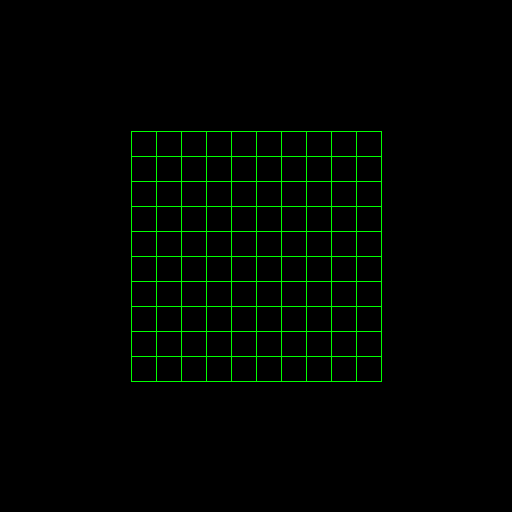
\includegraphics[trim={55 55 55 55},clip,scale=0.35]{original}  & 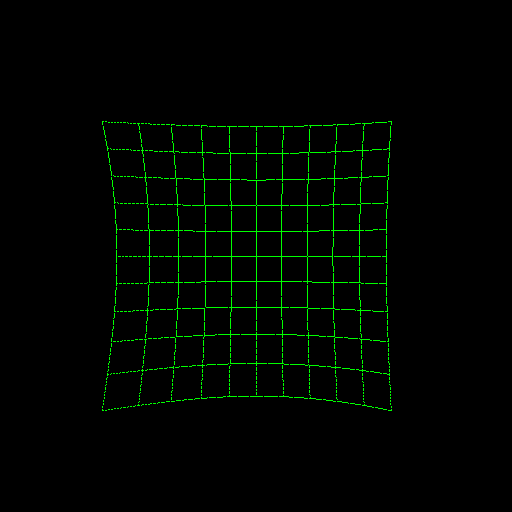
\includegraphics[trim={55 55 55 55},clip,scale=0.35]{distortionfull} \\
        ohne Verzeichnung & volle Verzeichnung \\
        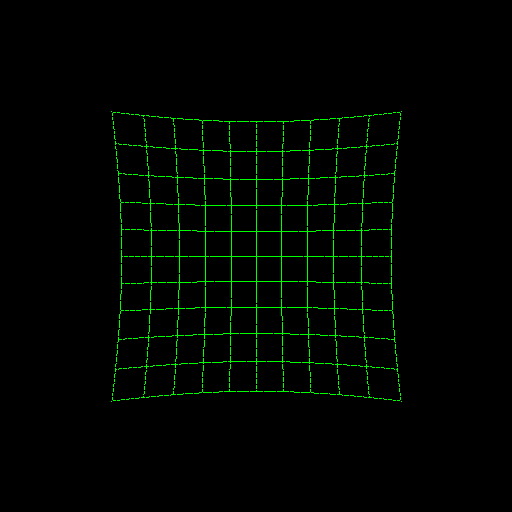
\includegraphics[trim={55 55 55 55},clip,scale=0.35]{distortionradial}  & 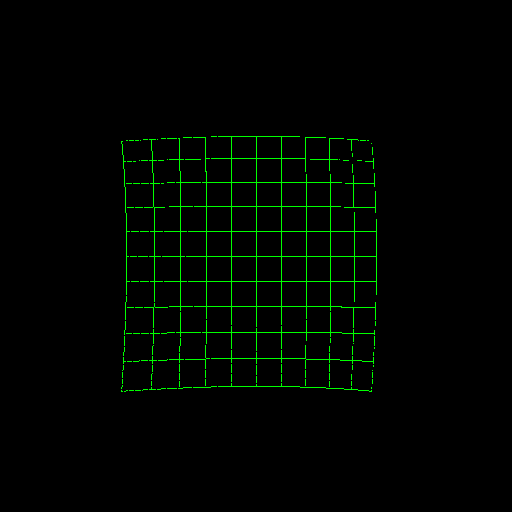
\includegraphics[trim={55 55 55 55},clip,scale=0.35]{distortiontangetial}  \\
        radiale Verzeichnung & tangentielle Verzeichnung
      \end{tabular}
    \end{table}
  \end{center}

\end{frame}

\begin{frame}<4>
  \frametitle{Unterschiedliche Arten von Parallelisierung}
  \framesubtitle{Bei der Parallelisierung sind zwei Begebenheiten zu unterscheiden}
  \begin{itemize}
    \item Datenparallelisierung - Aufteilen einer einzelnen Aufgabe
    \item Aufgabenparallelisierung - Aufteilen mehrerer von einander unabhängige Aufgaben
  \end{itemize}

\end{frame}

\begin{frame}<5>
  \frametitle{Ziel der Analyse}
  \framesubtitle{Bei der Aufteilung einer einzelnen Aufgabe}
  \begin{itemize}
    \item weniger Synchronisierungaufwand
    \item Vermeidung der Notwendigkeit zur Absicherung
    \item Isolierung einer Aufgabe  (divide and conquer)
    \item Kapselung für Fehlerfälle (Unhandled Exception)
  \end{itemize}

\end{frame}

\begin{frame}<6>
  \frametitle{Gegenüberstellung Platzproblem}
  \framesubtitle{Größe und Position vor und nach der Abbildung}
  Übersetzung von Texten:
  \begin{itemize}
    \item  Wann hört ein Satz auf? 
    \item  Wie groß ist er nach dem Übersetzen? 
    \item  Problemlösung: Tokenizer, jedoch auch eigene und neue Aufgabe
  \end{itemize}
  
  Pixelzugriff:
  \begin{itemize}
    \item  Besitzt einen absehbaren Iterator
    \item  $aktuelle Spalte+(Gesamtzahl Spalten*aktuelle Reihe) = wievielter Pixel$
    \item  oder auch: $d = Image.data(); d[wievielter Pixel]$
  \end{itemize}
  
\end{frame}

\begin{frame}<7>
  \frametitle{Selbststehende Aufgabe aufteilen}
  \framesubtitle{Die zu untersuchenden Eigenschaften}

  \begin{itemize}
    \item U ist die Menge der Ursprungspositionen im Speicher
    \item Z ist die Menge der Zielpositionen im Speicher
    \item $\digamma$ ist die Funktion, die U auf Z abbildet
  \end{itemize}

  \begin{itemize}
    \item Die Größe und Position eines jeden einzelnen Elementes der Eingabemenge ist bekannt
    \item Die Größe und Position eines jeden einzelnen Elementes der Ausgabemenge ist bekannt
    \item Die Bearbeitungszeit eines Elementes
  \end{itemize}

\end{frame}

\begin{frame}<8>
  \frametitle{Weitere Eigenschaften}
  \framesubtitle{}
  
  \begin{itemize}
    \item Ist die Positionsänderung eines Pixels injektiv, wird jeder Pixel aus U genau einem Pixel aus Z zugewiesen.
    \item ist die Positionsänderung eines Pixel dagegen surjektiv, kann ein Pixel aus Z durch mehrere Pixel aus U beschrieben werden.
  \end{itemize}
  
\end{frame}

\begin{frame}<9>
  \frametitle{Zwischenerkenntnisse}
  \framesubtitle{}
    
  \begin{center}
    Ist die Abbildungsfunktion der Position...
  \end{center}
  
  \begin{itemize}
    \item  injektiv, müssen nur ggfs. leere Positionen gefüllt werden.
    \item  surjektiv, müssen Ergebnisse zur gleichen Zielposition in einem zusätzlichen Konstrukt vorgehalten werden. Werden die Eingabeelemente verändert, so müssen diese auch vor Veränderung geschützt werden, bis alles berechnet wurde (vgl. Game of Life)
  \end{itemize}

  
\end{frame}

\begin{frame}<10>
  \frametitle{Beispiel: Skalierung eines Bildes}
  \framesubtitle{Halbierung des Bildes wird verwendet um in einer geringeren Datenmenge Bereiche auszuschließen}

  \begin{itemize}
    \item Pixel werden in einem n-Tupel gebündelt, wobei n eine endliche Zahl ist 
    \item Beispiel: Wird ein Bild halbiert, wird ein 4-Tupel auf ein 1-Tupel abgebildet. Dabei werden 2x2 Pixel zu einem zusammengefasst
  \end{itemize}
  
\end{frame}


\begin{frame}<11>
  \frametitle{Bearbeitungszeit einzelner Elemente}
  \framesubtitle{}
  
  \begin{itemize}
    \item Für die Bearbeitung einzelner Elemente kann eine Laufzeitanalyse durchgeführt werden
    \item Wenn es mehr zu bearbeitende Elemente als gleichzeitig laufende Threads existieren, so muss man sich Gedanken über die Aufteilung machen
  \end{itemize}

\end{frame}

\begin{frame}<12>
  \frametitle{Amdahlsches Gesetz}
  \framesubtitle{Geschwindigkeitsgewinn eines parallelisierbaren Problems}

  \begin{center}
    \begin{table}[]
      \begin{tabular}{ll}
        Formelzeichen & bezeichnete Größe \\
        T & Gesamtlaufzeit \\
        $t_s$ & Laufzeit eines seriellen Programmabschnitts \\
        $t_p$ & Laufzeit eines parallelen Programmabschnitts \\
        $n_p$ & Anzahl der nutzbaren Prozessoren \\
        $t_{O(np)}$ & Laufzeit für Synchronisierungsaufwand \\
        $n_s$ & Speedup-Faktor \\
      \end{tabular}
    \end{table}
  \end{center}
  
  \begin{center}
    \[ n_s = \dfrac{T}{t_s+t_{O(np)}+\dfrac{t_p}{n_p}} \leq \dfrac{T}{t_s} = \dfrac{T}{T-t_p} \]
  \end{center}
  
\end{frame}

\begin{frame}<13>
  \frametitle{Amdahlsches Gesetz}
  \framesubtitle{}

    \begin{itemize}
    \item  Die Funktion hat für jede Eingabe eine obere Schranke
    \item  Kann 50\% einer Aufgabe parallel zum restlichen Teil ausgeführt werden, ist die obere Schranke 2
    \item  Das Gesetz gbit eine schnelle Einschätzung über den Geschwindigkeitsgewinn
  \end{itemize}
  
\end{frame}

\begin{frame}<14>
  \frametitle{Parallelisierung einer For-Schleife}
  \framesubtitle{}
  
  \begin{itemize}
    \item  Ein absehbarer Iterator kann ich Chunks aufgeteilt werden
    \item  $aktuelle Spalte+(Gesamtzahl Spalten*aktuelle Reihe) = wievielter Pixel$
    \item  Jeder Chunk bekommt einen Start- und Endindex, so wie das notwendige Inkrement 
    \item  Die entstanden Chunks können auf einen einzelne Threads aufgeteilt werden
  \end{itemize}

\end{frame}

\begin{frame}<15>
  \frametitle{Aufgabenteilung in Chunks}
  \framesubtitle{Geschwindigkeitsgewinn eines parallelisierbaren Problems}
  
  \begin{center}
    \begin{table}[]
      \begin{tabular}{cc}
        
\includegraphics[scale=0.25]{chunksmall} & 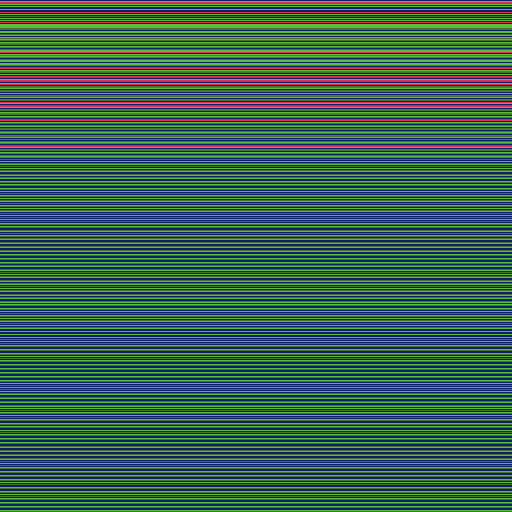
\includegraphics[scale=0.25]{chunkbig} \\
        Chunkgröße 5 Pixel & Chunkgröße Anzahl der Spalten 
      \end{tabular}
    \end{table}
  \end{center}

\end{frame}

\begin{frame}<16>
  \frametitle{Aufgabenteilung in Chunks}
  \framesubtitle{Geschwindigkeitsgewinn eines parallelisierbaren Problems}
  
  \begin{center}
    Mandelbrot mit 2048x2048 Pixeln und 4 Threads
  \end{center}
  
  \begin{center}
    \begin{table}[]
      \begin{tabular}{lrr}
        Art & Dauer in Sekunden & Speedup \\
        Sequentiell & 40,149 & - \\
        Breite*1 & 13,022 & 3,08 \\
        Breite*51 & 12,126 & 3,31
      \end{tabular}
    \end{table}
  \end{center}
  
  \begin{center}
    
\includegraphics[scale=0.0625]{mandelbrot}
  \end{center}

\end{frame}

\begin{frame}<17>
  \frametitle{Threadpools}
  \framesubtitle{}

    \begin{itemize}
    \item  Mehrere Threads werden in einem Objekt gekapselt
    \item  Die Threads sind in einem wartenden Zustand, bis neue Aufgaben kommen 
    \item  Objectpooling reduziert den Initialisierungsaufwand
    \item  Der Verwaltungsaufwand für Threads wird von der tatsächlichen Bearbeitung abgekapselt
  \end{itemize}
  
\end{frame}

\begin{frame}<18>
  \frametitle{Taskmanager ähnliches Konstrukt}
  \framesubtitle{kontrolliert eine begrenze Anzahl an Threads}

    \begin{itemize}
    \item  kontrolliertes Beenden des Programmes
    \item  verhindert größere Auslastung als vorgegeben
    \item  garantiert Bearbeitungszeit 
    \item  falls implementiert, umschalten zu sequentieller Bearbeitung (z.B. im Fehlerfall)
  \end{itemize}
  
\end{frame}

\begin{frame}<19>
  \frametitle{Literatur}
  \framesubtitle{}

    \begin{itemize}
    \item  Operating System Concepts, Abraham Silberschatz 
    \item  OpenMP Complete Specifications Version 3.1 – Jul 2011
    \item  Mikroprozessortechnik, Klaus Wüst 
    \item  Design Patterns, Erich Gamma
    \item  C++ Primer, Stanley B.Lippman
  \end{itemize}
  
\end{frame}

\end{document}
